\documentclass[xcolor=pdftext, table]{beamer}
\usepackage{amsmath, amssymb, amsfonts, latexsym, stmaryrd}
%\usepackage[latin1]{inputenc}
\usepackage[T1]{fontenc}
\usepackage[utf8]{inputenc}
\usepackage[english, spanish]{babel}
% Tabla de tres secciones
\usepackage[flushleft]{threeparttable}

% \toprule, \midrule, \bottomrule
\usepackage{booktabs}
% Tablas con ancho establecido por usuario
\usepackage{tabularx}

% Para diagramas de bloques entre otros
\usepackage{smartdiagram}
\usesmartdiagramlibrary{additions}

% Para vinculos a archivos externos
\usepackage{hyperref}

% tikz
\usepackage{tikz}
\usetikzlibrary{arrows.meta, positioning, shadows}

\usefonttheme{professionalfonts}
%\usetheme{Bergen}
%\usetheme{Hannover}
%\usetheme{Boadilla}
%\usetheme{Luebeck}
\usetheme{Warsaw}
%\usetheme{AnnArbor}

\setbeamercovered{transparent}

% Definicion de colores tabla cronograma
\definecolor{colorfa}{rgb}{0.3569,0.608,0.8353}
\definecolor{colorfb}{rgb}{0.4392,0.678,0.2784}
\definecolor{colorfc}{rgb}{1.0000,0.361,0.0000}
\definecolor{colorsem}{rgb}{0.1804,0.455,0.7098}
\definecolor{colorfd}{rgb}{0.9294,0.490,0.1922}
\definecolor{colorfe}{rgb}{0.2667,0.329,0.4157}

% Definicion comandos tabla cronograma
\newcommand{\fa}{\cellcolor{colorfa}}
\newcommand{\fb}{\cellcolor{colorfb}}
\newcommand{\fc}{\cellcolor{colorfc}}
\newcommand{\sem}{\cellcolor{colorsem}}
\newcommand{\fd}{\cellcolor{colorfd}}
\newcommand{\fe}{\cellcolor{colorfe}}
\newcommand{\fg}{\cellcolor{colorfa}}
\newcommand{\fj}{\cellcolor{colorfb}}

% Definicion de tipos de columnas tabla
\newcolumntype{C}[1]{>{\centering}m{#1}}
\newcolumntype{L}[1]{>{\raggedleft}m{#1}}
\newcolumntype{R}[1]{>{\raggedright}m{#1}}

\setbeamertemplate{headline}{}

\setbeamertemplate{footline}
{
	\leavevmode%
	\hbox{%
		\begin{beamercolorbox}[wd=.4\paperwidth,ht=2.25ex,dp=1ex,center]{author in head/foot}%
		\usebeamerfont{date in head/foot}\insertshortauthor
		\end{beamercolorbox}%
		\begin{beamercolorbox}[wd=.6\paperwidth,ht=2.25ex,dp=1ex,center]%
			{title in head/foot}%
			\usebeamerfont{title in head/foot}\insertshorttitle\hspace*{3em}
			\insertframenumber{} / \inserttotalframenumber\hspace*{1ex}
		\end{beamercolorbox}}%
	\vskip0pt%
}

\setbeamertemplate{note page}[plain]

\begin{document}
	\title{Seminario Trabajo Especial de Grado}
	
	\subtitle{\large DISEÑO DE UN EQUIPO ELECTRÓNICO CONTROLADOR DE
		INTERRUPTORES Y ATENUADORES EMPLEADO EN LA
		MEDICIÓN DE LA FIGURA DE RUIDO EN DISPOSITIVOS DE
		RADIO FRECUENCIA}
		
	\author{{\bf Jose Arias}\\
		%{Tutor: MSc. Pedro Ruiz}\\
		%{Prof. Guía: MSc. Alejandro González}
		}		
		
	\institute{Universidad Central de Venezuela \\
		Facultad de Ingeniería \\
		Escuela de Ingeniería Eléctrica \\
		Departamento de Electrónica, Computación y Control}
	
	\date{Febrero 2018}
	
	%\logo{\includegraphics[height=1.5cm]{Imagenes/pie-der.pdf}}

	\frame{\titlepage}
	
	\section{Planteamiento del Problema}
	
	\begin{frame}
		\frametitle{Sistema para medición de figura de ruido (SMFR)}	
	
		\begin{figure}		
			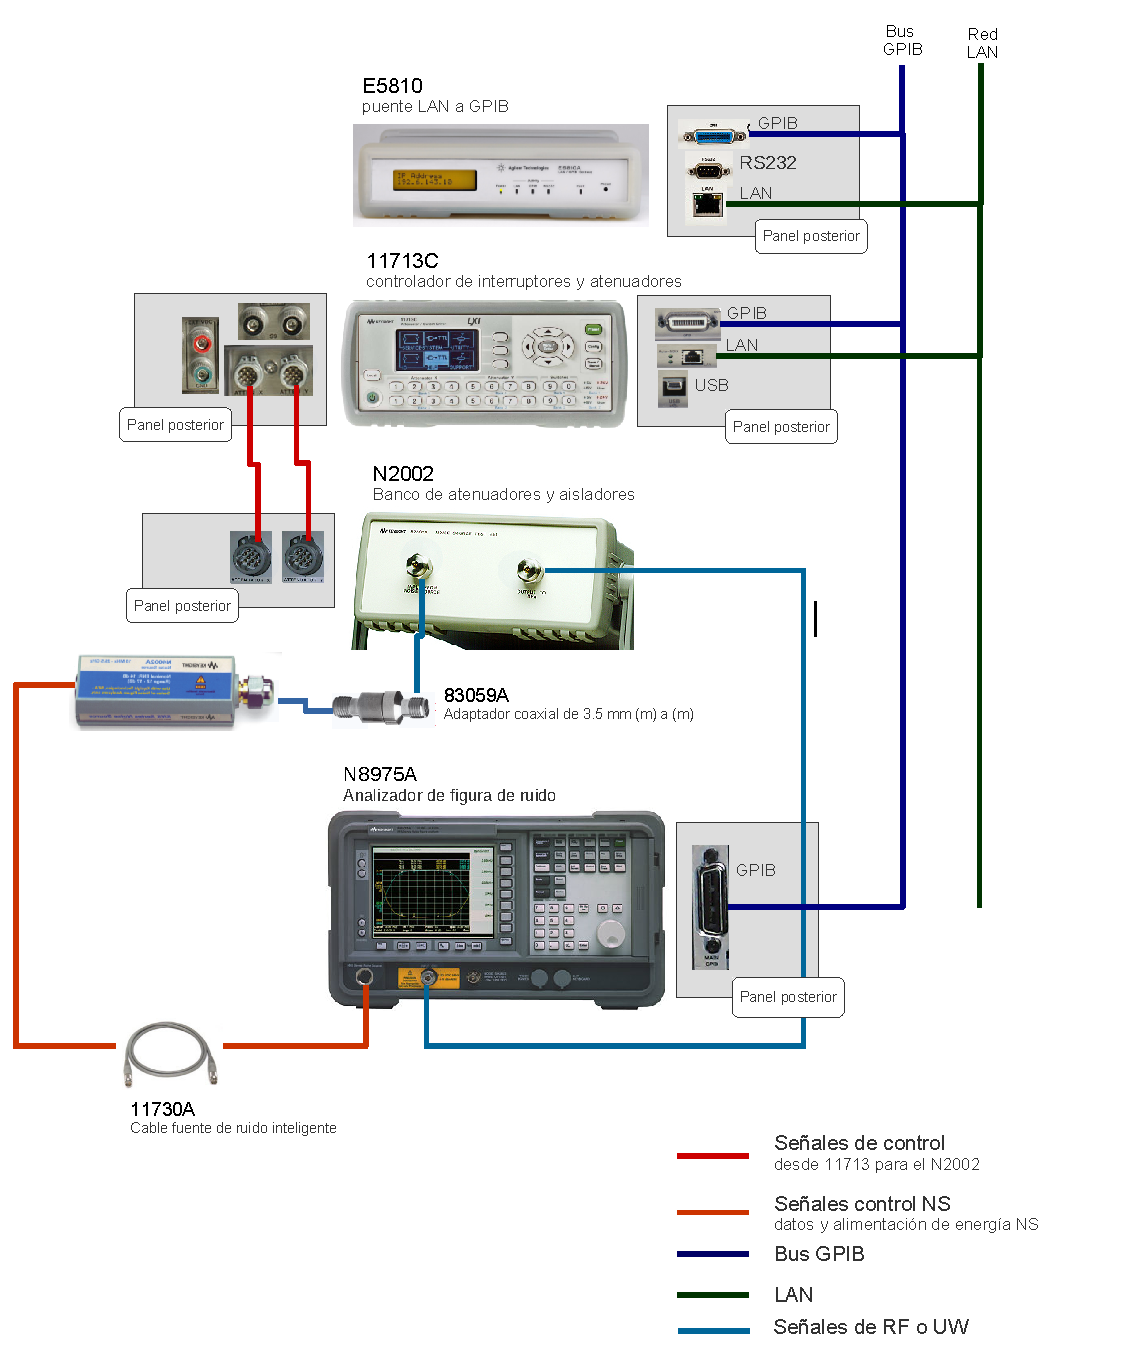
\includegraphics[height=4cm]{Imagenes/SistemaMedicionFiguraRuido.pdf}	
		\end{figure}			

		\begin{table}
			%\resizebox{\textwidth}{!}{
			\begin{tabular}{p{2cm}p{2cm}p{2cm}p{2cm}}
				\begin{minipage}{2cm}
					\includegraphics[width=2cm]{Imagenes/N8975A.pdf}
				\end{minipage} &	
				\begin{minipage}{2cm}
					\includegraphics[width=2cm]{Imagenes/N2002A.pdf}
				\end{minipage} &							
				\begin{minipage}{2cm}
					\includegraphics[width=2cm]{Imagenes/11713A.pdf}
				\end{minipage} &	
				\begin{minipage}{2cm}
					\includegraphics[width=2cm]{Imagenes/11713B.pdf}
				\end{minipage} \\
													
				{\scriptsize Analizador de figura de ruido (NFA) N8975A} &
				{\scriptsize Equipo para pruebas con fuente de ruido N2002A} &							
				{\scriptsize Controlador electrónico de interruptores y atenuadores, serie 11713} &
				{\scriptsize Controlador electrónico de interruptores y atenuadores, serie 11713} 
				
			\end{tabular}
			%}	
		\end{table}	
	\end{frame}

	\begin{frame}
		\frametitle{Panorama del SMFR}			
	
		\begin{figure}
			\begin{center}
				\includegraphics[width=10cm]{Imagenes/DiagramaBloquesSistema.pdf}
			\end{center}
		\end{figure}	
	
	\end{frame}
	
	\section{Objetivos} 
	
	\begin{frame}
		\frametitle{Objetivos}		
		
		\begin{block}{Objetivo general}
			\centering
			Diseñar un equipo electrónico que permita emular las características funcionales de un controlador electrónico de interruptores y atenuadores.
		\end{block}
		
		El título y el objetivo general permanecen sin cambios	
		
	\end{frame}
	
	\begin{frame}
		\frametitle{Objetivos}		

		\begin{small}
			\begin{block}{Objetivos específicos}		
				\begin{enumerate}
					\item Realizar una investigación documental sobre caracterización de dispositivos de radio frecuencia y la medición de figura de ruido en éstos.	
											
					\item Recopilar la documentación y software asociado al sistema de medición de figura de ruido (SFMR).	
					
					\item Codificar una librería de software para intercambio de datos entre PC y el SMFR.
					
					\item Diseñar y codificar el firmware para dispositivo.
					
					\item Diseñar y construir las tarjetas electrónicas PCB para cada uno de los módulos del equipo: expansor de puertos, fuente de alimentación y tarjeta madre. 
					
					\item Desarrollar una aplicación de software para gestión de la medición de figura de ruido con el SMFR.
					
					\item Generar manuales de usuario para el equipo y para la aplicación.	
				\end{enumerate}				
			\end{block}
		\end{small}
		
	\end{frame}
	
	\section{Alcance}
	
	\begin{frame}
		\frametitle{Cambios en el alcance}
		
		\begin{columns}
			\begin{column}{6cm}
				\begin{block}{Hardware}			
					\begin{itemize}				
						\item Interfaz de comunicaciones a través de USB. \\ 
						{\tiny (Class Device Communication, full speed).}
						{\tiny Inicialmente se habian propuesto las interfaces GPIB, USB, LAN}
		
						\item Señales para comandar la unidad de atenuadores y aisladores (N2002A) \\ 
						{\tiny formada por 2 grupos de 16 señales cada uno.}
								
						\item El panel frontal consistirá de un teclado matricial \\ 
						{\tiny Con 16 teclas.} 
						{\tiny Se elimina la pantalla LCD táctil}
					\end{itemize}
				\end{block}	
			\end{column}
			
			\begin{column}{6cm}
				\begin{figure}
					\begin{center}
						\includegraphics[width=6cm]{Imagenes/DiagramaBloquesSistema.pdf}
					\end{center}
				\end{figure}
			\end{column}			
		\end{columns}
		
	\end{frame}
	
	\begin{frame}
		\frametitle{Cambios en el alcance}
		
		\begin{block}{Software} 
			\begin{itemize}
				\item Instalador para la aplicación
				\item Soporte, a nivel de librerías de software, para establecer comunicación de datos con los dispositivos del sistema de medición de figura de ruido.
				\item Interfaz de usuario gráfica.
				\item Asistencia al usuario durante el ciclo de medición: configuración, ejecución y generación de reportes.
				\item Generación de reportes con resultados de una medición, en formato de documento portable (pdf).
			\end{itemize}	
		\end{block}
		
		
		\begin{block}{Firmware}
			\begin{itemize}
				\item Soporte a las comunicaciones por medio de las interfaz USB.
				\item Gestión de la interacción del usuario con el panel frontal. 	
			\end{itemize}
		\end{block}
		
	\end{frame}	

	\section{Metodología y Cronograma}
	
	\begin{frame}
		\begin{block}{Nuevo cronograma de trabajo}		
			\begin{threeparttable}[!h]
				\centering
				\arrayrulecolor{gray}
				\setlength{\extrarowheight}{4pt}		
				\resizebox{\textwidth}{!}{
					\begin{tabular}{|c|l|l|l|l|l|l|l|l|l|l|l|l|l|l|l|}
						\begin{tabular}{c}
							{\raggedright \textbf{Semanas}} \\
							\textbf{Tareas}
						\end{tabular}
						& 1 & 2 & 3 & 4 & 5 & 6 & 7 & 8 & 9 & 10 & 11 & 12 & 13 & 14 & 15\\
						\hline
						Expansor de puertos Viking & \fa & \fa & \fa & \fa & & & & & & & & & & & \\
						\hline				
						Firmware del dispositivo & & & & & & \fc & \fc & \fc & \fc & & & & & & \\ 
						\hline
						Tarjeta madre & & & & & & & & \fd & \fd & \fd & \fd &  & & & \\
						\hline
						Tarjeta de alimentación DC  &  & \fe & \fe & \fe & \fe & & & & & & & & & & \\
						\hline
						Desarrollo de la aplicación SGMFR  & & & & & & &  & \fg & \fg & \fg & \fg & \fg & \fg & \fg & \fg \\
						\hline
						Libro de TEG & & & & & & & & &  & \fj & \fj & \fj & \fj & \fj & \fj \\
						\hline
					\end{tabular}		
				}
				\begin{tablenotes}
					\item {\tiny Fecha de inicio: octubre de 2017.} 
					\item {\tiny Jornada de 8 horas diarias, lunes a viernes, de 8:00 AM a 12:00 M y de 1:30 PM a 4:30 PM.}
				\end{tablenotes}
			\end{threeparttable}		
		\end{block}			
	\end{frame}
	
	\begin{frame}
		\frametitle{Metodología de trabajo}
	
		\begin{block}{Cronograma inicial}
			\begin{threeparttable}[!h]
				\centering
				\arrayrulecolor{gray}
				\setlength{\extrarowheight}{4pt}		
				\resizebox{\textwidth}{!}{
					\begin{tabular}{|c|l|l|l|l|l|l|l|l|l|l|l|l|l|l|l|l|l|l|l|l|l|l|l|l|l|l|l|l|}
						\hline 			
						\textbf{Semanas} & 1 & 2 & 3 & 4 & 5 & 6 & 7 & 8 & 9 & 10 & 11 & 12 & 13 & 14 & 15 & 16 & 17 & 18 & 19 & 20 & 21 & 22 & 23 & 24 & 25 & 26 & 27 & 28 \\
						\hline
						\textbf{Fase 1}
						& \fa & \fa & \fa & \fa & \fa & \fa & & & & & & & & & & & & & & & & & & & & & & \\			
						\hline			
						\textbf{Fase 2} & & & & & & & \fb & \fb & \fb & \fb & \fb & \fb & \fb & \fb & \fb & \fb & \fb & & & & & & & & & & & \\
						\hline
						\textbf{Fase 3} & & & & & & & & & & & & & & & & & & \fc & \fc & \fc & \fc & \fc & & & & & & \\	
						\hline		
						\textbf{Seminario} & & & & & & & & & & & & & & \sem & & & & & & & & & & & & & & \\
						\hline
						\textbf{Fase 4} & & & & & & & & & & & & & & & & & & & & & & & \fd & \fd & \fd & \fd &  & \\
						\hline
						\textbf{Fase 5} & & & & & & & & & & & & & & & & & & & & & & & & & & & \fe & \fe \\
						\hline	
					\end{tabular}
				}
				\begin{tablenotes}
					\item {\tiny Fecha de inicio: 6 de Marzo de 2017.} 
					\item {\tiny Jornada de 8 horas diarias, lunes a viernes, de 8:00 AM a 12:00 M y de 1:30 PM a 4:30 PM.}
				\end{tablenotes}
			\end{threeparttable}
		
			\begin{itemize}
				\item Fase 1: Preparación y documentación.
				\item Fase 2: Diseño de dispositivo.
				\item Fase 3: Implementación de dispositivo.
				\item Fase 4: Producción de manual de usuario. 
				\item Fase 5: Documentación TEG. 				
			\end{itemize}
		
		\end{block}

	\end{frame}

	\section{Resumen de Tareas}
	
		\begin{frame}	
			\frametitle{Realizadas desde el último seminario}
			
			\begin{block}{Hardware}				
				\begin{columns}
					\begin{column}{6cm} 
						
						
						
					\end{column}
					\begin{column}{6cm} 
						Diseño y construcción de tarjetas PCB.
						Procura de componentes.
					\end{column}
				\end{columns}	
			\end{block}
		

			
			\begin{block}{Software}
				Aplicación funcional hasta interfaz de usuario.
			\end{block}
		
		\end{frame}

	\begin{frame}
		\frametitle{Documentación}
		
		\begin{itemize}
		 	\item Investigación sobre caracterización de dispositivos en alta frecuencia: parámetros de dispersión.
		 	\item Investigación sobre medición de figura de ruido en RF y microondas.
		 	\item Documentación acerca de cada uno de los instrumentos que integran el SMFR.
		 	\item Documentación acerca del software asociado o que brinda soporte al SMFR.				
		 \end{itemize}		

	\end{frame}

	\begin{frame}
		\frametitle{Tareas pendientes}	
			
			\begin{block}{Software}
				Culminar el diseño de la aplicación CenditLab
				\begin{itemize}
					\item Librerías de soporte de comunicaciones IO para Windows
					\item Culminar módulo gestión GUI
					\item Culminar módulos de gestión de instrumentos
					\item Culminar módulos de gestión de medición
				\end{itemize}
					
			\end{block}		

		\end{frame}
	
	\begin{frame}
	
	\frametitle{Tareas pendientes}		
	
		\begin{block}{Firmware}
			Iniciar el diseño y generación de firmware Cendit 11713
			\begin{itemize}
				\item Control de expansor de puertos Viking
				\item Comunicaciones por medio del bus USB
				\item Comunicaciones a través de redes LAN (TCP/IP)
				\item Gestión de la fuente de alimentación
				\item Gestión de la interfaz de usuario (teclado y pantalla)
			\end{itemize}
		\end{block}

	\end{frame}	

	\begin{frame}
		\frametitle{Tareas pendientes}			
	
		\begin{block}{Hardware}
			Culminar diseños, construcción y depuración para los módulos 
			\begin{itemize}
				\item Fuente de alimentación
				\item Teclado capacitivo
				\item Expansor de puertos Viking 
				\item Módulo Ethernet
				\item Pantalla LCD	
				\item Tarjeta madre				
			\end{itemize}
		\end{block}
	
	\end{frame}
\end{document}